\section{上界的评价}
\label{sec:tail-bound-comparison}

前面几节各自给出了一个界，每次都和精确值比了一比。现在把它们放在同一个变量、同一个阈值上，回答三个问题：每个界用了多少信息，在什么阈值上才有用，信息不全或矩不存在时还剩下什么。

\paragraph{同一事件上的排列}
对贯穿例子的事件$\{X\geq15\}$，表~\ref{tab:tail-bounds}列出各个界及其所需的信息。四阶、六阶矩界以$a=10$为中心，作用于包含$\{X\geq15\}$的双侧事件$\{\lvert X-10\rvert\geq5\}$；表的最后一行留到后面解释。

\begin{BookInlineTable}
 \centering
 \caption{$X\sim\operatorname{Bin}(20,1/2)$时$\mathbb{P}(X\geq15)$的精确值与各个上界。比值为上界除以精确值$0.0207$。}
 \label{tab:tail-bounds}
 \begin{tabular}{lllr}
  \toprule
  方法 & 所用信息 & 数值 & 比值\\
  \midrule
  精确值 & 完整质量表 & $0.0207$ & $1$\\
  Markov & $X\geq0$，$\mathbb{E}[X]=10$ & $0.667$ & $32$\\
  Chebyshev & $\mathbb{E}[X]$，$\operatorname{Var}(X)=5$ & $0.200$ & $9.7$\\
  四阶矩 & $m_4=72.5$ & $0.116$ & $5.6$\\
  六阶矩 & $m_6=1692.5$ & $0.108$ & $5.2$\\
  指数矩 & $M_X(\lambda)$，$\lambda>0$ & $0.0731$ & $3.5$\\
  最优原点矩 & $\mathbb{E}[X^k]$，$k\leq60$ & $0.0646$ & $3.1$\\
  \bottomrule
 \end{tabular}
\end{BookInlineTable}

图~\ref{fig:tail-bounds-bar}在对数刻度上画出同样的数。越往下，用到的信息越多，界越小，但即使是最好的界也比精确值大三倍。差距不会消失，因为每个界都是对一整类分布的保证：只要另一个分布与$X$有相同的已知数值而尾部更重，界就必须照顾它。

\begin{BookInlineFigure}
 \centering
 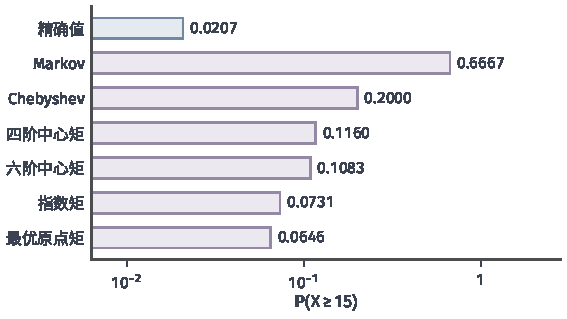
\includegraphics[width=96mm]{figures/07-probability/01-elementary-probability/matplotlib/tail-bounds-bar/figure.pdf}
 \caption{$X\sim\operatorname{Bin}(20,1/2)$时$\mathbb{P}(X\geq15)$的精确值（蓝）与各个上界（紫），横轴为对数刻度，数字为数值。四阶、六阶中心矩以$10$为中心；最优原点矩在$k=1,\dots,60$中取$\mathbb{E}[X^k]/15^k$的最小值，于$k=17$取到。}
 \label{fig:tail-bounds-bar}
\end{BookInlineFigure}

\paragraph{矩与指数矩的关系}
表中最后一行用的是原点矩$\mathbb{E}[X^k]$，对每个$k$由质量表求和，然后取$\mathbb{E}[X^k]/15^k$的最小值，在$k=17$处得到$0.0646$，竟比指数矩上界还小。这不是巧合：对非负变量，最好的矩上界从来不劣于指数矩上界。

\begin{theorem}[最优矩上界不劣于指数矩上界]
\label{thm:tail-moment-vs-chernoff}
设$Y\geq0$，$t>0$，$\lambda>0$且$M_Y(\lambda)<\infty$。则
\begin{equation}
 \inf_{k=0,1,2,\dots}\frac{\mathbb{E}[Y^k]}{t^k}\leq\mathrm{e}^{-\lambda t}M_Y(\lambda) .
 \label{eq:tail-moment-vs-chernoff}
\end{equation}
\end{theorem}

\begin{proof}
把$\mathrm{e}^{\lambda Y}$展成幂级数，各项$\lambda^kY^k/k!$都非负。非负项的级数可以与求和或积分交换次序，依据与引理~\ref{lem:tail-integral}证明中交换积分次序的依据相同，所以
\[
 M_Y(\lambda)=\sum_{k\geq0}\frac{\lambda^k\,\mathbb{E}[Y^k]}{k!} .
\]
两边乘$\mathrm{e}^{-\lambda t}$，并把每项写成“权重乘矩上界”：
\[
 \mathrm{e}^{-\lambda t}M_Y(\lambda)=\sum_{k\geq0}\Bigl(\mathrm{e}^{-\lambda t}\frac{(\lambda t)^k}{k!}\Bigr)\cdot\frac{\mathbb{E}[Y^k]}{t^k} .
\]
括号里的权重是参数为$\lambda t$的Poisson分布的质量，非负且和为$1$。记$b=\inf_k\mathbb{E}[Y^k]/t^k$，每个矩上界都不小于$b$，所以加权和不小于$b$：
\[
 \mathrm{e}^{-\lambda t}M_Y(\lambda)\geq b\sum_{k\geq0}\mathrm{e}^{-\lambda t}\frac{(\lambda t)^k}{k!}=b .
\]
这就是式~\eqref{eq:tail-moment-vs-chernoff}。
\end{proof}

证明说明了两者的关系：指数矩上界是各阶矩上界按Poisson权重的平均，平均值不会小于其中最小的一项。对右边取下确界后结论仍成立，所以式~\eqref{eq:tail-chernoff}的Chernoff界总不小于最优矩上界。定理要求$Y$非负，并且比较的是关于$0$的原点矩；对一般的$X$和单侧事件，可以取$Y=X$（当$X\geq0$时）或$Y=\lvert X-a\rvert$。

图~\ref{fig:tail-moment-vs-chernoff}在$Y=\lvert Z\rvert$、$Z\sim\mathcal{N}(0,1)$上验证这一点。$\lvert Z\rvert$的矩母函数为$2\mathrm{e}^{\lambda^2/2}\Phi(\lambda)$，其中$\Phi$是标准高斯分布函数，下确界需要数值计算。在$t=3$处，精确值、最优矩上界和指数矩上界依次为
\[
 0.0027,\qquad 0.0156,\qquad 0.0222 .
\]
两个界的差距不大，量级相同。

\begin{BookInlineFigure}
 \centering
 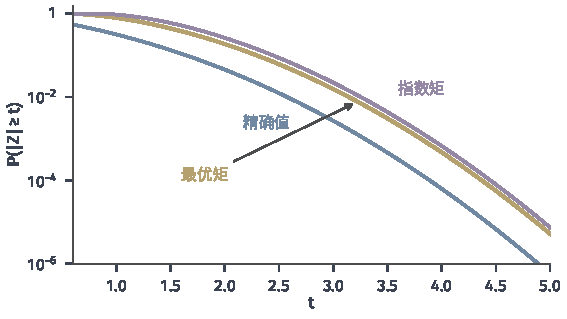
\includegraphics[width=96mm]{figures/07-probability/01-elementary-probability/matplotlib/tail-moment-vs-chernoff/figure.pdf}
 \caption{$Z\sim\mathcal{N}(0,1)$的$\mathbb{P}(\lvert Z\rvert\geq t)$（蓝线）、对实数阶$p>0$取最小的矩上界$\inf_p\mathbb{E}\lvert Z\rvert^p/t^p$（黄线）与$\lvert Z\rvert$的指数矩上界$\inf_{\lambda>0}\mathrm{e}^{-\lambda t}M_{\lvert Z\rvert}(\lambda)$（紫线），纵轴为对数刻度。}
 \label{fig:tail-moment-vs-chernoff}
\end{BookInlineFigure}

既然矩上界更紧，为什么还要指数矩？原因在计算。最优矩上界要求知道全部各阶矩，再对阶数搜索；指数矩把它们压缩成一个函数，常常有闭式，例如二项分布的$\bigl((1+\mathrm{e}^{\lambda})/2\bigr)^{20}$，只需一维最小化。对独立量之和，矩母函数还能分解成乘积，而高阶矩的展开会迅速变得繁琐。

\paragraph{反过来求试验次数}
界的差距在反问题中看得更清楚。掷$n$次均匀硬币，正面次数$X\sim\operatorname{Bin}(n,1/2)$，正面比例是$X/n$。要使比例偏离$1/2$至少$0.1$的概率不超过$0.05$，$n$至少要多大？

先用Chebyshev不等式。由第~\ref{chap:common-distributions}章，$\operatorname{Var}(X)=n/4$；由缩放规律，$\operatorname{Var}(X/n)=1/(4n)$。于是
\[
 \mathbb{P}\Bigl(\Bigl\lvert\frac{X}{n}-\frac12\Bigr\rvert\geq0.1\Bigr)\leq\frac{1/(4n)}{0.01}=\frac{25}{n} .
\]
要使右边不超过$0.05$，需要$n\geq500$。

再用指数矩上界。右侧事件是$\{X\geq0.6n\}$，在式~\eqref{eq:tail-binomial-chernoff-general}中取$p=1/2$，$a=0.6$，方括号里的数是
\[
 \Bigl(\frac{0.5}{0.6}\Bigr)^{0.6}\Bigl(\frac{0.5}{0.4}\Bigr)^{0.4}=\mathrm{e}^{-0.02014}\approx0.9801 .
\]
由对称性左侧事件$\{X\leq0.4n\}$有同样的界，两侧相加得$2\mathrm{e}^{-0.02014n}$。令它不超过$0.05$，解得$n\geq\ln40/0.02014\approx183.2$，即$n\geq184$。

最后用质量表直接计算。精确概率随$n$的变化并不单调，因为$0.6n$是否为整数会影响端点上的质量：$n=97$时约为$0.0417$，$n=100$时又升到$0.0569$。逐个计算可知，从$n=106$起精确概率都不超过$0.05$（数值检查到$n=500$）。三种方法给出的次数是$500$、$184$与$106$。上界越紧，为同一个保证付出的试验次数越少；精确计算最省，但要对每个$n$求和，而且只适用于确知的分布。

\paragraph{有效阈值}
每个界只在一段阈值上提供信息，在其余阈值上不小于$1$。Markov界在$t\leq\mathbb{E}[X]$时不小于$1$；Chebyshev界在$t\leq\sigma$时不小于$1$。指数矩上界在$t\leq\mathbb{E}[X]$时也给不出信息：由第~\ref{chap:random-variable-moments}章的Jensen不等式，$\mathrm{e}^{\lambda x}$是凸函数，所以
\[
 \mathrm{e}^{-\lambda t}M_X(\lambda)\geq\mathrm{e}^{-\lambda t}\mathrm{e}^{\lambda\mathbb{E}[X]}=\mathrm{e}^{\lambda(\mathbb{E}[X]-t)}\geq1,\qquad \lambda>0 .
\]
这符合直觉：阈值不在均值右边时，“越过阈值”并不是一个罕见事件。实际使用时把每个界与$1$取较小者，例如写成$\min\{1,\mathbb{E}[X]/t\}$；图中所有的界都已这样截断。

\paragraph{重尾模型}
对$\alpha=3$的Pareto分布，指数矩不存在，三阶及以上的矩也不存在，能用的只有$p<3$阶的矩。由$\mathbb{E}[X^p]=3/(3-p)$，原点矩上界是
\[
 \mathbb{P}(X\geq t)\leq\frac{3}{(3-p)\,t^{p}},\qquad 0<p<3 .
\]
$p$越接近$3$，$t^{-p}$衰减越快，但系数$3/(3-p)$越大。对给定的$t$，把对数$\ln3-\ln(3-p)-p\ln t$对$p$求导并令其为零：
\[
 \frac{1}{3-p}-\ln t=0,\qquad p^{*}=3-\frac{1}{\ln t} .
\]
当$t>\mathrm{e}^{1/3}\approx1.40$时$p^{*}\in(0,3)$，二阶导数$1/(3-p)^2>0$，这是最小点。

代回去，$3-p^{*}=1/\ln t$，$t^{-p^{*}}=t^{-3}\,t^{1/\ln t}=\mathrm{e}\,t^{-3}$，于是
\begin{equation}
 \inf_{0<p<3}\frac{3}{(3-p)\,t^{p}}=\frac{3\mathrm{e}\ln t}{t^{3}},\qquad t>\mathrm{e}^{1/3} .
 \label{eq:tail-pareto-best}
\end{equation}
精确值是$t^{-3}$，最好的原点矩上界多出一个因子$3\mathrm{e}\ln t$，随$t$缓慢增大。$t=10$时，界为$0.0188$，精确值为$0.001$。图~\ref{fig:tail-pareto-moments}在双对数坐标中画出这些曲线：每个固定阶数的界是一条斜率为$-p$的直线，红色虚线是它们的下包络。

\begin{BookInlineFigure}
 \centering
 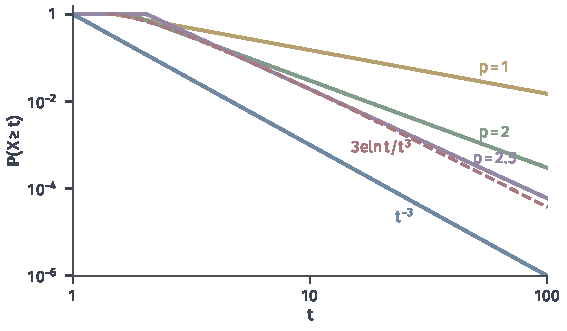
\includegraphics[width=96mm]{figures/07-probability/01-elementary-probability/matplotlib/tail-pareto-moments/figure.pdf}
 \caption{$\alpha=3$的Pareto分布，双对数坐标。蓝线为精确尾部$t^{-3}$，黄、绿、紫线为$p=1,2,2.5$的原点矩上界$\min\{1,3/((3-p)t^p)\}$，红色虚线为对$p\in(0,3)$取最小的包络$3\mathrm{e}\ln t/t^3$。}
 \label{fig:tail-pareto-moments}
\end{BookInlineFigure}

中心的选择同样重要。Pareto分布的均值为$3/2$，方差为$3-9/4=3/4$。对$t>3/2$，事件$\{X\geq t\}$包含在$\{\lvert X-3/2\rvert\geq t-3/2\}$中，Chebyshev不等式给出$\tfrac34/(t-\tfrac32)^2$。$t=10$时这是$0.0104$，反而比式~\eqref{eq:tail-pareto-best}的$0.0188$更好；$t=100$时它是$7.7\times10^{-5}$，又不如后者的$3.8\times10^{-5}$。以均值为中心去掉了原点处的偏移，在中等阈值上更有利；阈值很远时，阶数的作用占了上风。

更重的尾部会让可用的工具进一步减少。Cauchy分布连均值都没有，Markov不等式和Chebyshev不等式都不能用，只剩阶数$p<1$的绝对矩上界。这时尾概率本身也只按$1/t$衰减，任何依赖高阶矩的估计都无从谈起。

\paragraph{信息与代价}
图~\ref{fig:tail-information-ladder}把本章的界按所需信息排列。越往下，假设越强：均值有限弱于方差有限，方差有限弱于更高阶矩有限，而某个$\lambda>0$处指数矩有限蕴含一切阶矩有限。假设越强，界越紧，适用的分布越少。完整分布在最下面，它给出精确值，但需要的信息最多，计算也可能最难，例如高斯尾部$Q(t)$就要数值积分。

\begin{BookInlineFigure}
 \centering
 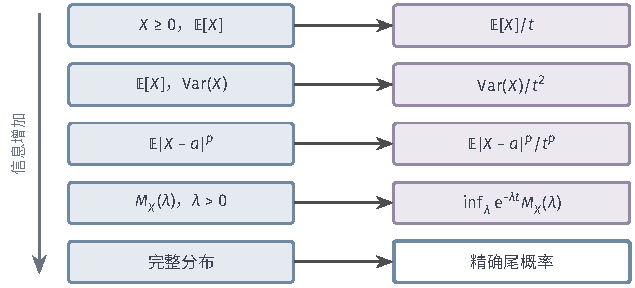
\includegraphics[width=108mm]{figures/07-probability/01-elementary-probability/tikz/tail-information-ladder/figure.pdf}
 \caption{所用信息（左）与得到的尾部结论（右）。前两行分别控制$\mathbb{P}(X\geq t)$与$\mathbb{P}(\lvert X-\mathbb{E}[X]\rvert\geq t)$，第三行控制$\mathbb{P}(\lvert X-a\rvert\geq t)$，第四行控制$\mathbb{P}(X\geq t)$。自上而下大致按所需的矩条件由弱到强排列，紫色为上界，白色为精确值。}
 \label{fig:tail-information-ladder}
\end{BookInlineFigure}

计算成本按相反方向排列。Markov界和Chebyshev界只要一两个数，一次除法；矩上界要计算一个积分或求和；指数矩上界要先得到矩母函数，再做一维最小化，可以求导，也可以数值搜索；精确值要对整个尾部求和或积分。实际选择时先问手上有什么信息，再问需要多紧的保证。

\paragraph{保证与估计}
最后要分清三种数。精确尾概率是具体分布的性质。Markov界和Chebyshev界在各自的信息下是最好的保证，第~\ref{sec:tail-markov}节和第~\ref{sec:tail-chebyshev}节的极端分布达到了它们，所以不能指望仅凭这些信息改进。矩上界与指数矩上界则依赖额外的假设：高阶矩或指数矩存在，并且已知其数值。额外的假设换来了更紧的界，也缩小了适用范围；假设一旦不成立，例如遇到重尾模型，就要退回到弱的界。
